%*************************************************************************
%* Copyright © 2012-2014 Vincent Prat & Simon Nicolas
%*
%* This document is free; you can redistribute it and/or modify
%* it under the terms of the GNU General Public License as published by
%* the Free Software Foundation; either version 3 of the License, or
%* (at your option) any later version.
%*
%* This document is distributed in the hope that it will be useful,
%* but WITHOUT ANY WARRANTY; without even the implied warranty of
%* MERCHANTABILITY or FITNESS FOR A PARTICULAR PURPOSE. See the
%* GNU General Public License for more details.
%*
%* You should have received a copy of the GNU General Public License along
%* with this document; if not, write to the Free Software Foundation, Inc.,
%* 51 Franklin Street, Fifth Floor, Boston, MA 02110-1301 USA.
%*************************************************************************

\documentclass[a4paper,12pt]{article}

\usepackage[frenchb]{babel}
\usepackage[utf8]{inputenc}
\usepackage{graphicx}
\usepackage{hyperref}
\usepackage{xspace}

\graphicspath{{images/}}

\newcommand*{\GMA}{GM-Assistant\xspace}
\newcommand*{\interfaceitem}[1]{\texttt{#1}}
\newcommand*{\guillemets}[1]{\og #1\fg{}\xspace}
\newcommand*{\versionnumber}{1.2\xspace}

\title{\GMA \versionnumber, guide de l'utilisateur}
\author{Simon Nicolas \and Vincent Prat}
\date{18 décembre 2014}

\begin{document}

\maketitle

\tableofcontents

\section{Introduction}

Une partie de jeu de rôle est une alchimie riche et complexe.
Les joueurs doivent être impliqués et investis et le maître de jeu (ou MJ) doit parfaitement maîtriser le système de règle, le scénario, se rappeler des évènements précédents, anticiper les évènements à venir, et improviser le présent en fonction des actions et choix des joueurs.
Si en pleine partie le MJ doit chercher des détails sur un personnage, une précision sur un point de règle, des musiques d'ambiance ou des bruitages sur l'ordinateur, des images dans son classeur, ou autre, alors la partie ralentit, l'émulsion retombe, et les joueurs se dispersent.
Ne niez pas, un rôliste se disperse vite.

La solution est \GMA, pour \emph{Game Master Assistant} (en français, assistant au MJ).
Son objectif est de simplifier la vie du MJ en mettant à sa disposition les informations et outils dont il peut avoir besoin pendant la partie.
\GMA propose donc une interface où le MJ va pouvoir rassembler et ordonner toutes les informations, notes et fichiers (musiques, bruitages, images) qu'il estime utiles.

Cette documentation a pour but d'aider l'utilisateur (c'est-à-dire vous) à se familiariser avec le logiciel.
La fenêtre principale du logiciel comporte d'une part une barre de menus, qui sera développée dans la section~\ref{menu} et d'autre part 6 sous-parties que nous appellerons modules et qui seront présentés dans la section~\ref{sec:modules}.
Le logiciel propose également un certain nombre d'outils annexes qui feront l'objet de la section~\ref{sec:outils}.
Pour finir, en cas de besoin, vous pourrez trouver la liste des raccourcis clavier dans l'annexe~\ref{sec:raccourcis}. 

\section{Présentation des menus}
\label{menu}

La barre de menus de \GMA est similaire à celle que l'on trouve dans la plupart des logiciels.
Nous allons maintenant détailler un par un les menus principaux, qui sont \interfaceitem{Jeu} (section~\ref{sec:jeu}), \interfaceitem{Édition} (section~\ref{sec:edition}), \interfaceitem{Affichage} (section~\ref{sec:affich}), \interfaceitem{Outils} (section~\ref{sec:menu_outils}) et \interfaceitem{Aide} (section~\ref{sec:aide}).

\subsection{Jeu}
\label{sec:jeu}

Ce menu comprend tous les outils de gestion et de sauvegarde des fiches de scénarios créées avec \GMA.
En voici la liste~:
\begin{description}
    \item[\interfaceitem{Nouveau}~:]{crée une nouvelle fiche de scénario vide}
    \item[\interfaceitem{Recharger}~:]{restaure la fiche de scénario courante telle qu'elle était lors de la dernière sauvegarde}
    \item[\interfaceitem{Charger}~:]{charge une fiche de scénario stockée dans un fichier}
    \item[\interfaceitem{Récents}~:]{propose la liste des fiches de scénario récemment ouvertes}
    \item[\interfaceitem{Enregistrer}~:]{sauvegarde la fiche de scénario en cours d'édition}
    \item[\interfaceitem{Enregistrer sous}~:]{sauvegarde la fiche de scénario en cours d'édition dans un nouveau fichier}
    \item[\interfaceitem{Métadonnées}~:]{affiche une fenêtre permettant de noter le titre du scénario, son auteur, la date de création, une description sommaire, le jeu de rôle, la liste des joueurs et la date de jeu.
            L'idée est de rassembler des informations qui ne servent pas pendant la partie mais qui permettent de se souvenir de \guillemets{Qui~? Quand~? Comment~?}.}
    \item[\interfaceitem{Quitter}~:]{ferme la fiche de scénario en cours et quitte le logiciel}
\end{description}
\paragraph{Le fichier de sauvegarde}
Le fichier de sauvegarde \texttt{.gms} créé est un fichier complet qui comprend toutes les informations qui sont dans la fiche de scénario et les fichiers annexes que vous y avez ajouté (musique, bruitages, images), lui permettant d'être déplacé d'un ordinateur à un autre sans risque de perte (un son manquant ou une image absente par exemple).

\subsection{Édition}
\label{sec:edition}

Ce menu a pour but d'aider l'utilisateur lors de l'élaboration de la fiche de scénario.
Pour l'instant, il se compose uniquement de deux actions~:
\begin{description}
    \item[\interfaceitem{Annuler}~:]{annule la dernière modification apportée}
    \item[\interfaceitem{Refaire}~:]{rétablit la dernière modification apportée après son annulation}
\end{description}

\subsection{Affichage}
\label{sec:affich}

Ce menu permet de choisir parmi différentes options d'affichage.
Il se compose de deux sous-menus~:
\begin{description}
    \item[\interfaceitem{Interface}~:]{ouvre la liste des arrangements de modules disponibles (voir la section~\ref{sec:modules} pour la description de chacun des modules).
        Chaque interface propose un appariement différent de modules~:
        \begin{description}
            \item[\interfaceitem{Complète}~:]{est composée des 6 modules}
            \item[\interfaceitem{Simple}~:]{est composée des modules \interfaceitem{Intrigue}, \interfaceitem{Musique} et \interfaceitem{Bruitage}}
            \item[\interfaceitem{Musique}~:]{est composée des modules \interfaceitem{Musique} et \interfaceitem{Bruitage}}
            \item[\interfaceitem{Conception}~:]{est composée des modules \interfaceitem{Intrigue}, \interfaceitem{Personnages} et \interfaceitem{Notes}}
            \item[\interfaceitem{Sans son}~:]{est composée des modules \interfaceitem{Intrigue}, \interfaceitem{Historique}, \interfaceitem{Personnages} et \interfaceitem{Notes}}
        \end{description}
    }
    \item[\interfaceitem{Langue}~:]{ouvre la liste des langues disponibles pour l'interface graphique du logiciel.
        Actuellement, seuls l'anglais et le français sont supportés.}
\end{description}

\subsection{Outils}
\label{sec:menu_outils}

Ce menu rassemble les différents outils annexes proposés par \GMA.
Le fonctionnement de ces outils sera abordé en détail dans la section~\ref{sec:outils}.
Dans la présente version du logiciel, le menu comprend~:
\begin{description}
    \item[\interfaceitem{Simulateur de dés}~:]{permet de simuler le lancer d'un certain nombre de dés d'un certain type}
    \item[\interfaceitem{Gestionnaire de combat}~:]{outil permettant de structurer le déroulement des combat}
\end{description}

\subsection{Aide}
\label{sec:aide}

Ce menu donne accès aux informations générales sur le logiciel et sa licence.

\section{Présentation des modules}
\label{sec:modules}

Comme évoqué précédemment, la fenêtre principale du logiciel est découpée en six modules indépendants et dédiés chacun à une fonctionnalité.
Plusieurs de ces modules se présentent sous forme d'un arbre \guillemets{dépliable} permettant d'organiser des informations.
Les possibilités offertes par ces arbres et les items qui les composent seront développées dans la section~\ref{item}.
Voici la liste des modules présents dans cette version~:
\begin{description}
    \item[\interfaceitem{Intrigue}~:]{arbre qui permet d'afficher de manière ordonnée les différents évènements important du scénario (voir la section~\ref{sec:intrigue} pour plus de détail)}
    \item[\interfaceitem{Historique}~:]{encore un arbre, qui a cette fois vocation à rappeler les évènements les plus marquants des scénarios précédents ou du passé des personnages (voir section~\ref{sec:historique})}
    \item[\interfaceitem{Notes}~:]{éditeur de texte simpliste qui permet de prendre des notes avant ou pendant la partie (voir section~\ref{sec:notes})}
    \item[\interfaceitem{Personnages}~:]{tableau permettant d'afficher les protagonistes avec leurs caractéristiques importantes (voir section~\ref{sec:perso})}
    \item[\interfaceitem{Musique}~:]{lecteur de musique simple pensé pour jouer des musiques d'ambiance (voir section~\ref{sec:musique})}
    \item[\interfaceitem{Bruitages}~:]{lecteur de musique encore plus simple pensé pour jouer des bruitages courts (voir section~\ref{sec:bruitages})}
\end{description}
Tout ces modules sont rassemblés dans l'interface par défaut du logiciel, comme on peut le voir sur la figure~\ref{fig:interface}, mais peuvent également être réorganisés grâce au sous-menu \interfaceitem{Interface} du menu \interfaceitem{Affichage} décrit précédemment dans la section~\ref{sec:affich}.
\begin{figure}[ht]
    \centerline{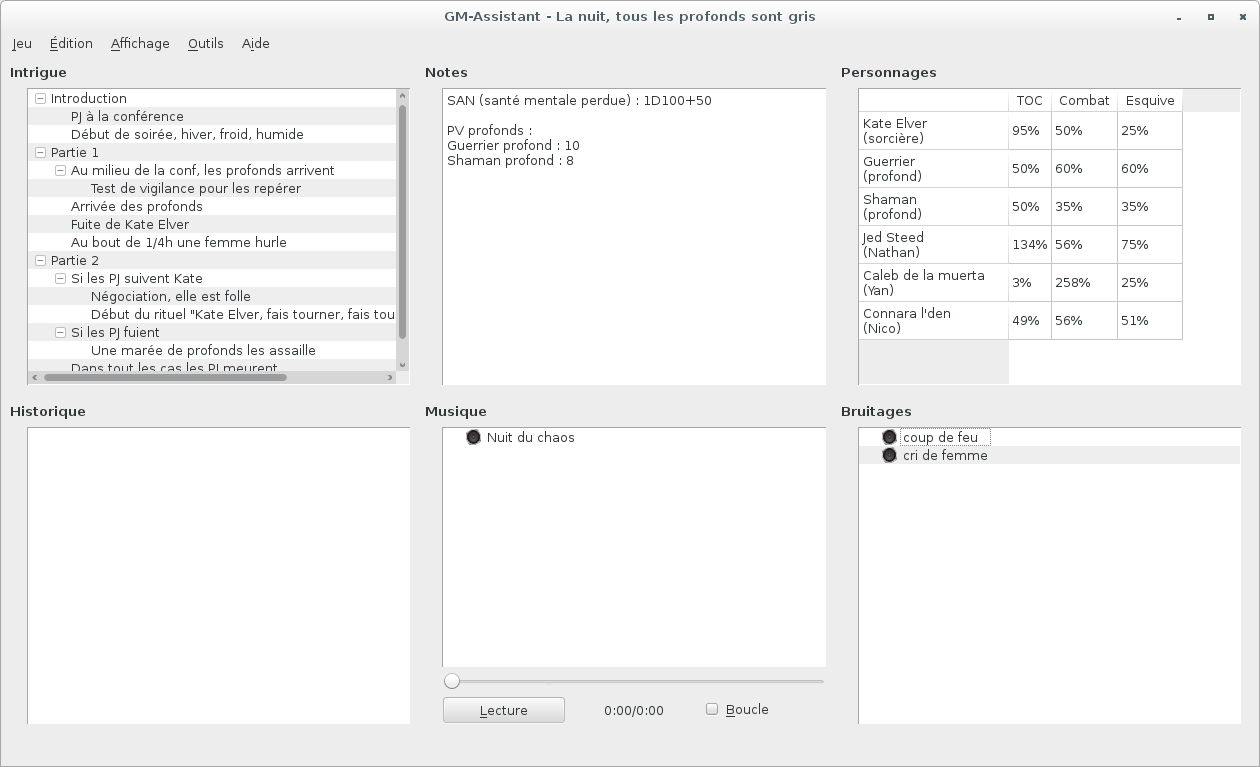
\includegraphics[width=0.9\textwidth]{scenario_complet}}
    \caption{Fenêtre principale du logiciel avec une partie en cours}
    \label{fig:interface}
\end{figure}

\subsection{La notion d'item}
\label{item}

Les items sont à la base du fonctionnement de \GMA, il est donc approprié d'en expliquer le fonctionnement avant de détailler les modules.
Par définition, un item désigne un élément minimal d'un ensemble.
Dans notre cas, un item est une ligne, une entrée dans un des modules sous forme d'arbre du logiciel, qui sert à contenir une information textuelle, un son (musique ou bruitage), une image, etc.
Les modules qui utilisent les items sont \interfaceitem{Intrigue}, \interfaceitem{Historique}, \interfaceitem{Musique} et \interfaceitem{Bruitage}.

Chaque item se présente comme une ligne de texte, à laquelle est associé un état qui permet de prendre rapidement note du succès ou de l'échec de certains points clefs du scénario et d'en avoir une vision rapide.
Les quatre états disponibles sont \interfaceitem{Aucun}, \interfaceitem{En cours}, \interfaceitem{Échoué} et \interfaceitem{Réussi}.
Un item peut également comporter du contenu supplémentaire, selon son type, qui peut être \interfaceitem{Basique} (aucun contenu supplémentaire), \interfaceitem{Audio} (musiques et bruitages) ou \interfaceitem{Image} (n'importe quel type d'image).

Lorsque vous cliquez avec le bouton droit de la souris sur un item apparaît le menu de gestion d'item.
Ce menu contient les quatre états possible d'un item puis les trois actions \interfaceitem{Ajouter}, \interfaceitem{Supprimer} et \interfaceitem{Éditer}.
Si l'item est de type \interfaceitem{Audio} ou \interfaceitem{Image}, une action supplémentaire est présente pour jouer le fichier audio ou afficher l'image.
Veuillez noter que pour les fichiers audio, cette action n'apparaît que dans les modules \interfaceitem{Musique} et \interfaceitem{Bruitages}.

L'action \interfaceitem{Ajouter} nous permet d'accéder à la fenêtre de création d'item (figure~\ref{fig:ajout}).
\begin{figure}[ht]
    \centerline{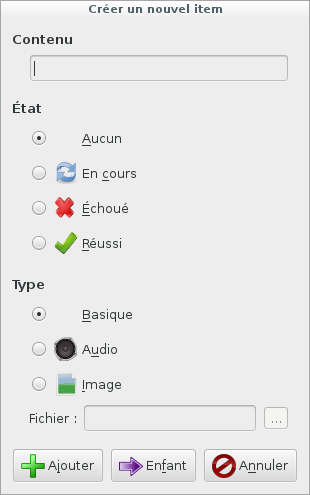
\includegraphics[width=0.5\textwidth]{add_item}}
    \caption{Fenêtre de création d'item}
    \label{fig:ajout}
\end{figure}
Notez qu'il est également possible d'accéder à cette fenêtre en cliquant avec le bouton droit de la souris dans la partie vide du module ou en appuyant sur la touche \interfaceitem{Inser} de votre clavier.
Voici comment s'organise cette fenêtre~:
\begin{itemize}
    \item le cadre \interfaceitem{Contenu} reçoit la description de l'évènement~;
    \item le cadre \interfaceitem{État} permet de fixer l'état de l'item~;
    \item le cadre \interfaceitem{Type} permet de choisir le type de l'item et pour les items de type \interfaceitem{Audio} et \interfaceitem{Image} de sélectionner le fichier correspondant~;
    \item Le bouton \interfaceitem{Ajouter} ajoute l'item à la suite et au même niveau que l'item sur lequel on a cliqué avant d'ouvrir la fenêtre (si aucun item n'était sélectionné, ajoute simplement l'item à la suite au niveau le plus bas)~;
    \item Le bouton \interfaceitem{Enfant} ajoute l'item à la suite et sous l'item sur lequel on a cliqué précédemment, imbriqué dedans~;
    \item Le bouton \interfaceitem{Annuler} annule la création d'item en cours.
\end{itemize}
Il est important de bien saisir la différence entre les deux boutons \interfaceitem{Ajouter} et \interfaceitem{Enfant}, car c'est grâce à eux que vous organiserez les étapes de votre scénario.
Une fois créés, les items sont également déplaçables au sein d'un même module par \guillemets{glisser-déposer}.

L'action \interfaceitem{Éditer} ouvre une fenêtre similaire à celle de création d'item, la seule différence importante étant qu'il n'y a plus \interfaceitem{Ajouter} et \interfaceitem{Enfant}, mais uniquement un bouton \interfaceitem{Valider} permettant de valider l'édition.
Si vous voulez uniquement modifier le texte d'un item, il vous suffit d'appuyer sur la touche \interfaceitem{F2} de votre clavier (la combinaison \interfaceitem{Ctrl+F2} ouvre quant à elle la fenêtre d'édition).

\subsection{Intrigue}
\label{sec:intrigue}

L'arbre d'intrigue est dans la majorité des cas le cœur de \GMA.
C'est en effet à cet endroit que vous pouvez entrer le plan détaillé et ordonné du scénario, de manière à ne jamais être perdu entre deux scènes ni oublier un élément.
La figure~\ref{arbre_scenar} donne un aperçu de ce qu'il est possible de faire avec ce module.
\begin{figure}[ht]
    \centerline{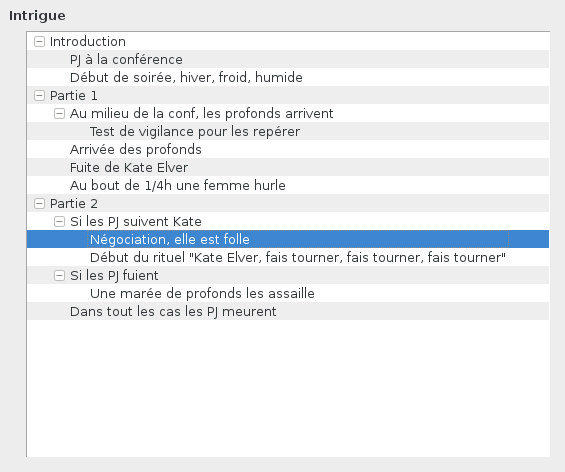
\includegraphics[width=0.6\textwidth]{scenario_type}}
    \caption{Plan schématique d'un scénario}
    \label{arbre_scenar}
\end{figure}
Chaque ligne que vous voyez est un item, et il suffit donc de suivre la technique de création d'item présentée dans la section~\ref{item} pour ordonner son scénario.
N'oubliez pas que vous pouvez modifier l'état des différents items composant l'intrigue au fur et à mesure que la partie avance pour garder une trace de la progression des personnages incarnés par vos joueurs (appelés PJ, par opposition aux PNJ, incarnés par le MJ).
Cela peut s'avérer utile si le scénario s'étale sur plusieurs séances.

\subsection{Historique}
\label{sec:historique}

L'arbre d'historique sert à préparer une liste des évènements importants ayant marqué les séances précédentes, commme les rencontres des personnages, une promesse faite par un PJ à un PNJ (ou l'inverse), etc.
Il est également possible d'y inscrire des éléments du passé des personnages.
De cette manière, toutes ces informations seront accessibles rapidement au MJ.
D'un point de vue technique, il se comporte et s'utilise exactement de la même manière que l'arbre d'intrigue.

\subsection{Notes}
\label{sec:notes}

Le module de prise de notes est un éditeur de texte simpliste (pour entrer du texte il suffit de cliquer avec le bouton gauche de la souris quelque part dans l'éditeur et d'écrire) qui permet de noter à la volée toute information utile à garder.
Par exemple~: \guillemets{Sylvain a insulté le directeur du museum}.
Ce module peut également être utilisé lors de la préparation d'une partie pour compléter certains éléments du scénario --- comme l'intrigue, l'historique ou encore les personnages --- avec des informations dont la longueur n'est pas adaptée aux modules correspondants.
Par exemple, il est possible d'y écrire la description d'un personnage que les PJ rencontrent, ou une histoire qui leur est racontée par un PNJ.

\subsection{Personnages}
\label{sec:perso}

Le module \interfaceitem{Personnages} est pensé pour accueillir la liste des protagonistes ainsi que les informations dont vous pourriez avoir besoin rapidement en cours de partie les concernant.
Ces informations, appelées \guillemets{propriétés} dans le logiciel, peuvent se présenter sous forme de nombres ou sous forme de texte.
Dans le module, les personnages correspondent à des lignes, et les propriétés à des colonnes.

De la même manière que pour les modules sous forme d'arbre, la construction du tableau se fait à l'aide du clic droit de la souris.
Cela affiche un menu déroulant permettant de choisir l'action voulue.
Lorsque le module est vide, les sous-menus \interfaceitem{Personnages} et \interfaceitem{Propriétés} permettent d'ajouter un personnage ou une propriété grâce à l'action \interfaceitem{Ajouter}.
Une fenêtre s'ouvrira alors, vous permettant de créer le personnage ou la propriété.
Dans le cas d'un personnage, outre son nom, vous aurez la possibilité d'ajouter une courte description permettant de l'identifier facilement.

Une fois qu'au moins un personnage et une propriété ont été créés apparaissent des cases éditables où l'on peut introduire les valeurs des différentes propriétés pour chaque personnage.
Cliquer avec le bouton droit de la souris dans une de ces cases ouvrira le même menu déroulant que précédemment, avec en plus la possibilité de supprimer ou d'éditer le personnage ou la propriété correspondant.
Notez qu'une fois un personnage ou une propriété créé, un clic droit sur le bandeau d'en-tête correspondant (horizontal pour les propriétés et vertical pour les personnages) ouvrira directement le sous-menu correspondant.

\subsection{Musique}
\label{sec:musique}

Le module de musique est un lecteur de musique basique qui permet de jouer des musiques d'ambiance ou des sons continus (comme de la pluie ou du vent).
Notez qu'il n'est possible de jouer qu'un seul morceau à la fois.

Le module se divise en deux parties : un arbre similaire à l'\interfaceitem{Intrigue} et à l'\interfaceitem{Historique} permettant de hiérarchiser les différents morceaux, et le lecteur proprement dit, composé de~:
\begin{itemize}
    \item une barre de défilement ainsi qu'un compteur qui indiquent la position dans le morceau en cours~;
    \item un bouton qui permet de contrôler la lecture~;
    \item une case à cocher permettant de jouer en boucle le morceau en cours.
\end{itemize}
Lorsqu'il n'y a pas de lecture en cours, il est écrit \interfaceitem{Lecture} sur le bouton.
Cliquer dessus joue le morceau sélectionné dans l'arbre.
Lors de la lecture, le texte du bouton est \interfaceitem{Pause}.
Cliquer dessus met alors la lecture en pause et le texte du bouton devient \interfaceitem{Reprise}.
Cliquer à nouveau reprend la lecture là où elle s'était arrêtée.
Faire glisser le curseur de la barre de défilement permet de naviguer dans le morceau.

\subsection{Bruitages}
\label{sec:bruitages}

Le module de bruitages est un lecteur de musique encore plus basique pensé pour jouer des sons très courts comme un coup de feu, un hurlement, une porte qui claque, \emph{etc.}
Contrairement au module de musique, celui des bruitages ne comporte qu'un arbre.
Pour jouer un bruitage, il suffit d'effectuer un double clic sur l'item audio voulu.

Il est tout à fait possible de jouer un bruitage alors qu'une musique est en cours de lecture.
En revanche, jouer un autre bruitage remplace immédiatement le bruitage en cours.
Une autre différence par rapport au module de musique est qu'une fois un bruitage en cours de lecture, il n'est pas possible de l'arrêter.

\section{Présentation des outils}
\label{sec:outils}

Tout comme les modules, les outils ont pour but de faciliter le travail du MJ lors de parties, mais contrairement à eux, ils ne servent pas à stocker d'informations.
Les deux outils disponibles dans la présente version du logiciel sont un simulateur de dés (voir section~\ref{sec:des}) et un gestionnaire de combat (voir section~\ref{sec:combat}).

\subsection{Simulateur de dés}
\label{sec:des}

Le simulateur de dés est un outil permettant de simuler directement dans le logiciel le résultat aléatoire de dés virtuels.
Vous aurez ainsi tout ce qu'il vous faut si vous avez oublié vos dés ou si vous voulez en lancer plus à la fois que ce dont vous disposez.
Pour l'utiliser, il suffit de sélectionner l'option correspondante du menu \interfaceitem{Outils}.
Une fenêtre similaire à celle représentée sur la figure~\ref{simulateur_des} s'ouvre alors.
\begin{figure}[ht]
    \centerline{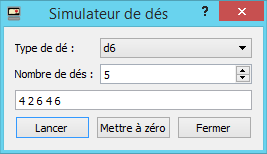
\includegraphics[width=0.6\textwidth]{simulateur_de_des}}
    \caption{Simulateur de dés}
    \label{simulateur_des}
\end{figure}

Cette fenêtre permet de choisir les éléments suivants :
\begin{description}
    \item[\interfaceitem{Type de dé}~:]{nombre de faces de chaque dé. Pour ceux qui ne seraient pas familiers avec les notations des rôlistes, d$n$ désigne un dé à $n$ faces.}
    \item[\interfaceitem{Nombre de dés}~:]{nombre de dés à lancer, jusqu'à concurrence de dix.}
\end{description}
Un simple clic sur le bouton \interfaceitem{Lancer} affiche le résultat donné par chacun des dés.
Le bouton \interfaceitem{Mettre à zéro} permet quant à lui d'effacer le résultat de lancers précédents.
Enfin, le bouton \interfaceitem{Fermer} sert à fermer le simulateur de dés une fois les lancers terminés.
Notez que toute l'interface du logiciel reste accessible même lorsque le simulateur est ouvert.

\subsection{Gestionnaire de combat}
\label{sec:combat}

Dans la plupart des jeux de rôle, les combats sont un peu compliqués à gérer.
En effet, il faut garder en mémoire l'ordre dans lequel les différents personnages agissent pour être capable de dire à tout moment qui doit agir.
Il faut également compter les points de vie des intervenants, les éventuelles blessures, \emph{etc.}
Pour aider le MJ dans cette tâche parfois difficile, \GMA propose un outil conçu à cet effet~: le gestionnaire de combat.

Tout comme pour le simulateur de dés, le gestionnaire de combat s'ouvre en sélectionnant l'option correspondante dans le menu \interfaceitem{Outils}.
Son utilisation se divise en deux étapes~: la sélection des participants au combat dans un premier temps, puis le combat proprement dit.

\subsubsection{Sélection des participants}

La première fenêtre à apparaître ressemble à celle représentée sur la figure~\ref{gestion_combat_choix}.
\begin{figure}[ht]
    \centerline{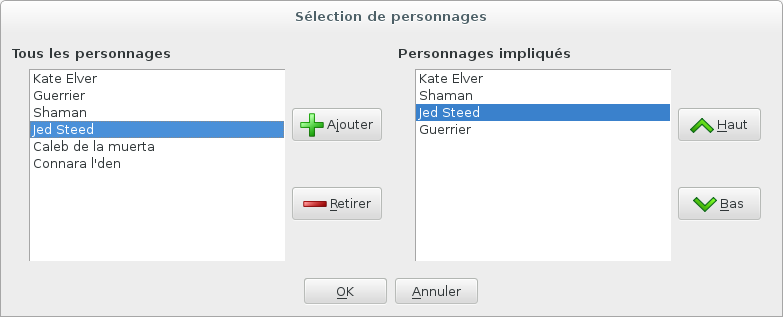
\includegraphics[width=1\textwidth]{gestionnaire_combat_prep}}
    \caption{Gestionnaire de combat~: sélection des participants}
    \label{gestion_combat_choix}
\end{figure}
La liste des personnages de la colonne de gauche est générée automatiquement à partir des protagonistes entrés dans le module \interfaceitem{Personnages}.
Il s'agit alors de choisir chaque participant au combat en le sélectionnant dans la colonne de gauche et en l'ajoutant à la colonne de droite en cliquant sur \interfaceitem{Ajouter}.
En cas d'erreur, il est possible de retirer de la colonne de droite un personnage en le sélectionnant et en cliquant sur \interfaceitem{Retirer}.

L'ordre dans lequel les différents acteurs figurent dans la colonne de droite est celui dans lequel ils agiront lors du combat.
Veillez donc à bien ordonner la liste des participants en utilisant les boutons \interfaceitem{Haut} et \interfaceitem{Bas}, qui ont pour effet de monter et descendre le personnage sélectionné dans la liste.
Sachez toutefois qu'il sera possible de changer l'ordre d'action en cours de combat.
Une fois la préparation terminée, il suffit de cliquer sur \interfaceitem{OK} pour passer à l'étape suivante.

\subsubsection{Combat}

Apparaît maintenant le gestionnaire de combat lui-même, représenté sur la figure~\ref{gestion_combat_fight}.
\begin{figure}[ht]
    \centerline{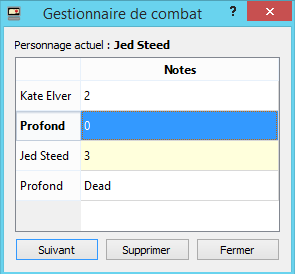
\includegraphics[width=0.4\textwidth]{gestion_combat_fight}}
    \caption{Gestionnaire de combat~: action}
    \label{gestion_combat_fight}
\end{figure}
On y retrouve la liste ordonnée de participants élaborée lors de l'étape précédente, avec en plus la possibilité d'ajouter une note pour chaque personnage dans la colonne \interfaceitem{Notes}.
Cela peut s'avérer utile pour noter les blessures, les points de vie actuels, ou encore tout autre commentaire spécifique.
Pour ce faire, il suffit de double-cliquer dans la case correspondante ou de taper \interfaceitem{F2} une fois la case sélectionnée.
Le fonctionnement du gestionnaire est le suivant~: à chaque tour de combat la ligne \interfaceitem{Personnage actuel} indique quel personnage doit agir.
La case de note du personnage en question apparaît alors sur fond jaunâtre.
Lorsque ce personnage a fini d'agir, on clique sur \interfaceitem{Suivant} et le gestionnaire passe au personnage suivant.

En cas de sortie du combat d'un personnage, par exemple en cas de fuite ou de mort, ce personnage peut être retiré simplement du gestionnaire en cliquant sur \interfaceitem{Supprimer} après l'avoir sélectionné.
Si au cours du combat un personnage décide de retarder son action, ou si vous vous êtes trompé dans l'ordre d'action lors de la phase de sélection des participants, il est possible de déplacer un personnage au sein de la liste par glisser-déposer.
Si c'était à ce personnage d'agir, le personnage suivant sera automatiquement sélectionné.
Enfin, une fois le combat terminé, il suffit de cliquer sur \interfaceitem{Fermer}.

\section{Conclusion}\label{conclusions}
\GMA est un logiciel conçu par des rôlistes pour des rôlistes, c'est-à-dire vous.
Si ce n'est déjà fait, nous vous encourageons à l'essayer.
S'il vous plaît, que vous n'envisagez plus de jouer sans, tant mieux.
Si pour une raison ou une autre ce n'est pas le cas, sachez que nous faisons de notre mieux.
Dans tous les cas, vous êtes cordialement invités à participer à l'amélioration de ce logiciel et ce de plusieurs façons, selon vos compérences et votre motivation~:
\begin{itemize}
    \item en utilisant le logiciel, en nous faisant part de vos impressions, et en signalant d'éventuels bogues~;
    \item en le faisant connaître autour de vous~;
    \item en proposant des fonctionnalités qui pourraient être intégrées à \GMA dans l'avenir~;
    \item en nous aidant à rédiger et relire la documentation~;
    \item en traduisant le logiciel et la documentation dans des langues qui ne sont pas encore supportées~;
    \item en maintenant à jour notre site web \url{http://gmassistant.free.fr}~;
    \item et enfin en rejoignant notre équipe de développeurs.
\end{itemize}

Si vous êtes intéressé, vous pouvez nous joindre à l'adresse \url{gmassistant@free.fr}.
Si vous posséder un compte Github, vous pouvez également suivre l'avancement du projet, jeter un coup d'œil au code et signaler des bogues sur la page du projet \url{http://github.com/ViviCoder/GM-Assistant}.
Enfin, si vous désirez être tenu au courant des dernières actualités concernant GM-Assistant, vous pouvez vous abonner à notre flux RSS (en anglais) \url{http://gmassistant.free.fr/feed}.

\appendix

\section{Liste des raccourcis clavier}
\label{sec:raccourcis}

\subsection{Menus}

\begin{description}
    \item[\interfaceitem{Ctrl+B}~:]{Gestionnaire de combat}
    \item[\interfaceitem{Ctrl+D}~:]{Simulateur de dés}
    \item[\interfaceitem{Ctrl+M}~:]{Métadonnées}
    \item[\interfaceitem{Ctrl+N}~:]{Nouveau jeu}
    \item[\interfaceitem{Ctrl+O}~:]{Charger}
    \item[\interfaceitem{Ctrl+Q}~:]{Quitter}
    \item[\interfaceitem{Ctrl+R}~:]{Recharger}
    \item[\interfaceitem{Ctrl+S}~:]{Enregistrer}
    \item[\interfaceitem{Ctrl+Maj+S}~:]{Enregistrer}
    \item[\interfaceitem{Ctrl+Z}~:]{Annuler}
    \item[\interfaceitem{Ctrl+Maj+Z}~:]{Refaire}
    \item[\interfaceitem{F1}~:]{À propos}
    \item[\interfaceitem{F5}~:]{Interface complète}
    \item[\interfaceitem{F6}~:]{Interface simple}
    \item[\interfaceitem{F7}~:]{Interface avec musique}
    \item[\interfaceitem{F8}~:]{Interface de conception}
    \item[\interfaceitem{F9}~:]{Interface sans son}
\end{description}

\subsection{Arbres}

\begin{description}
    \item[\interfaceitem{Espace}~:]{Jouer (musique ou son) ou afficher (image)}
    \item[\interfaceitem{Inser}~:]{Ajouter}
    \item[\interfaceitem{Suppr}~:]{Supprimer}
    \item[\interfaceitem{+}~:]{Déplier}
    \item[\interfaceitem{-}~:]{Replier}
    \item[\interfaceitem{F2}~:]{Édition simple}
    \item[\interfaceitem{Ctrl+F2}~:]{Édition complète}
    \item[\interfaceitem{Ctrl+F5}~:]{État \interfaceitem{Aucun}}
    \item[\interfaceitem{Ctrl+F6}~:]{État \interfaceitem{En cours}}
    \item[\interfaceitem{Ctrl+F7}~:]{État \interfaceitem{Échoué}}
    \item[\interfaceitem{Ctrl+F8}~:]{État \interfaceitem{Réussi}}
\end{description}

\subsection{Tableau}

\begin{description}
    \item[\interfaceitem{Ctrl+Inser}~:]{Ajouter une propriété}
    \item[\interfaceitem{Ctrl+Maj+Inser}~:]{Ajouter un personnage}
    \item[\interfaceitem{Suppr}~:]{Effacer une cellule}
    \item[\interfaceitem{Ctrl+Suppr}~:]{Supprimer une propriété}
    \item[\interfaceitem{Ctrl+Maj+Suppr}~:]{Supprimer un personnage}
    \item[\interfaceitem{F2}~:]{Éditer une cellule}
    \item[\interfaceitem{Ctrl+F2}~:]{Éditer une propriété}
    \item[\interfaceitem{Ctrl+Maj+F2}~:]{Éditer un personnage}
\end{description}

\end{document}
